\chapter{Hardware Implementation}

% **************************** Define Graphics Path **************************
\ifpdf
    \graphicspath{{Chapter3/Figs/Raster/}{Chapter3/Figs/PDF/}{Chapter3/Figs/}}
\else
    \graphicspath{{Chapter3/Figs/Vector/}{Chapter3/Figs/}}
\fi

The following sections shows us an overview about the hardware implementation of the Invariant Observer Design.
At first we get a description about the hardware platform on which the observer runs and some details
about the synthesis tools.
At the end of this chapter, there comes a design view about the synthesized hardware and a discussion about 
the design steps.
\section{Hardware Platform for a Prototype}
The Invariant Observer is synthesized on a Field Programmable Gate Array(FPGA),on this platform it was possible to get an insight
about the runtime behaviour and to see the observers in action. 
The FPGA Board that was used for the simulations is a \textbf{DE2-115} Board from ALTERA\cite{altera1}.
This FPGA Board is ideal to illustrate fundamental concepts and advanced designs,and it gives us a possibiliy
to meet the necessary real-time requirements we need. The DE2-115 is equipped with a \textbf{Cyclone IV EP4CE115F29} 
FPGA Chip and it is powerful enough to emulate a CPU(Nios).In \cite{RTFMBJ13} this Fpga board was used for performance studies,besides other FPGA's,
so it was logical to use a similar environment.
The Board has an onboard oscillator of 50 Mhz,and with the use of a Phase Locked Loop(PLL) it is possible to increase the working frequency for tests.
In the following section we will see how the increase of the frequency changes the design on Register Transfer level(RTL) and why bad design decisions 
can influence the maximal speed of the design. In Appendix~\ref{appendix:3} there is an schema illustration about the components of that FPGA board.


\section{Synthesis and Design}
This section gives us an overview about the synthesis tool and details about the Register Transfer Level design view.
An interesting part in this section is to see how the synthesis tool creates hardware structures based on the code of the
Observer VHDL implementation.\newline
For synthesis and compilation of the observer vhdl code ,the \textbf{Altera Quartus II Version 12.1 Build 177 Full Version} was used.
\subsection{Design View of the Register Transfer Level}
In Quartus II ,after compilation of the design and after creation of the netlists,you can use a tool,named \textbf{RTL Viewer},which shows how
the components of the design will be created on a Hardware Platform. It is an abstract view on the \textbf{Register Transfer Level}.
This tool can be very handy if you want to see how the hardware should look like. Based on the illustration of the hardware,some decisions can
be reconsidered in the meaning of the performance. \newline
Figure~\ref{fig:test:only:50:obs0} is a hardware plan of a single observer stage (m=1),which is modeled as a single Observer with input frequency of 50Mhz.
How the test system was modeled for that case,will be discussed in the next chapter.
The next Figure~\ref{fig:test:only:150:obs0} shows exact the same design case like Figure~\ref{fig:test:only:50:obs0} but with the difference that the input frequency is 150Mhz.
Here we can see how the synthese tool reorientates the hardware design,to meet the requirements of that clock speed. The worst case path determines the maximum frequency,which can drive
that design. 
A more detail description about the timing model is in the next subsection.
\subsection{Timing Model of the Design}
One important thing that have to be considered is that the signal path from the beginning of the observer entity to the end should be as short as possible.
Let's overview some important design facts.\newline
The maximum frequency of the whole system is determinded by the longest path of the design. This results that the performance of a system is determined by the maximum frequency
it can be driven. It is logical that,at every entity in the netlist,the path should be as short as possible.
The performance maximum can be computed by the Quartus Tool named \textbf{TimeQuest Timing Analyzer},which gives estimations about the maximum frequency of the design.
The ĺongest signal path of the design is indicated by the \textbf{worst case path} in the tool,as mentioned in the last subsection. \newline
The first version of the observer stage had a low performance niveau. This version is illustrated in the Appendix~\ref{fig:version:one:obs}.
The TimeQuest Timing Analyzer consider some uncertainties for the performance estimations.From \cite{altera2} we know how the Quartus Tool creates timing models which are
build in the TimeQuest Timing Analyzer after compilation of that design.
A Fpga have to operate in a continuum of conditions. These conditions include the die junction temperature,which varies.
Commercial parts have a range of 0°C to 85°C and industrials a bigger range. 
A second condition aspect is the voltage supply level. Critical voltages for maintaining FPGA performance is the Vcc and the various I/O supplies.
\newline
The timing analyzer shows estimations for three cases
\begin{enumerate}
\item Slow 1200mv 85°C model
\item Slow 1200mv 0°C model
\item Fast 1200mv 0°C model
\end{enumerate}

The operating-condition corners are usually the combinations of end points of the ranges in temperature, voltage and manufacturing processes.
Each operating-condition is used to model the timing delays under specific end point of temperature, voltage, and manufacturing process conditions.
The first case with ''Slow 1200mv 85°C model'' seems natural and should be considered for our test cases, because it shows frequencies under long term 
operating conditions.
A lot of tests about estimations of the maximum frequency of different design cases,are always took from that ''Slow 1200mv 85°C model'',and have to be considered
for further discussions.In the next chapter these tests will be discussed.

\subsection{Design Decisions based on Register Transfer level}

After the first time,the VHDL Code of the observer stage was behavioural correct,some perfomance and optimization decisions had to be reconsidered.
The most important thing is to separate synchronous and asynchronous design.At the beginning,it was necessary to split a completely synchronous design,where
every action is triggered after every clock cycle.A more parallel approach has to be done where only state changes are done synchronously,but other actions should
be triggered immediately after a change of a system state.And the asychronous system part can seperated in several independent asynchronous components,which achieves more 
system parallelism and a better performance.It should be mentioned again,from chapter 2,that this system design is similar to a moore state machine,where the logic 
is seperated in a transition logic,an output logic,and a state memory.And only the state memory is changed on every clock cycle.\newline
Our design approach of the invariant observer is similar,but with the difference that the output logic contains transition logic components.
The hardware schemas from the Register Transfer Level plans where beneficial,because it shows which components where created from the vhdl background.
If statements should be created in a way,that allow no Latches.This means that every else branch should contain the same components like the if branch.
If you follow that rule,you can see for example the created mutexes in Figure~\ref{fig:test:only:50:obs0}.Every mutex has two inputs(according to if,else),which are
selected depending on the third input(MUX21).\newline
At the beginning of the entity ther are several adders,and these stands for the different addition 
which has to be done according to the behaviour of the observer.\textbf{Add2} emulates $cycle\_next=cycle+1$ ,\textbf{Add1} emulates "$cycle\_next=cycle-1$" and \textbf{Add3}\\ 
emulates "$count\_p=count\_p+1$" according to the sourcecode of the Observer Stages in Appendix~\ref{appendix:source:2}.
In Figure~\ref{fig:test:only:50:obs0},the MUX 21 a the beginning indicated by \textbf{cycle\_next[15..0]} is the if branch ,according sourcecode in Appendix~\ref{appendix:source:2},
which decides if "$cycle=0$" or not. \newline
The \textbf{MUX21[cycle\_next[31..16]]} below stands for the branch "if $cycle=observernumber$".
\textbf{MUX21[cycle\_next[15..0]]} decrements cycle\_next in normal case,but increments it only once at the bottom border. 
\textbf{MUX21[cycle\_next[31..16]]} works the opposite way.
As you can see, the tool enhanced cycle\_next up to 48bit to reserver memory for 
interim results. \newline
In the hardware scheme,there are two another \textbf{MUX21[cycle\_next[15..0]]},the first(left to right) decides between  "$cycle\_next=cycle+1$" or "$cycle\_next=cycle-1$" and the second 
between that resultling decision before and the reset value.\textbf{MUX21[cycle\_next[47..32]]} decides between keeping the old value "$cycle\_next=cycle$" or 
taking over the value from \textbf{MUX21[cycle\_next[31..16]]}.The overview is similar to count\_p,but a deeper insight about the Quartus translation behaviour would exceed that subsection.
As you can see in the hardware schema, there are 5 registers(cycle,count\_p,direction,output,enable\_out) and these representate the state of the Invariant Observer and they only change their values
after every clock\_cycle. 
The dimensions of the registers are conform to the dimensions of the input conditions.
For example if inc\_tau has a value with only 5 bits,then count\_p is accodrdingly large-dimensioned to 6 Bit. 
This is only a cut-out,about how the Quartus II translate the incoming VHDL Code.
A lot of other hardware representations are shown in Appendix~\ref{appendix:2},actually they have the same components but another orientations.
The next subsection shows us something about the problems I had during the progress of that development.

\begin{figure}[]
\centering
%\hspace{3.0cm}
%\vspace{-5cm}
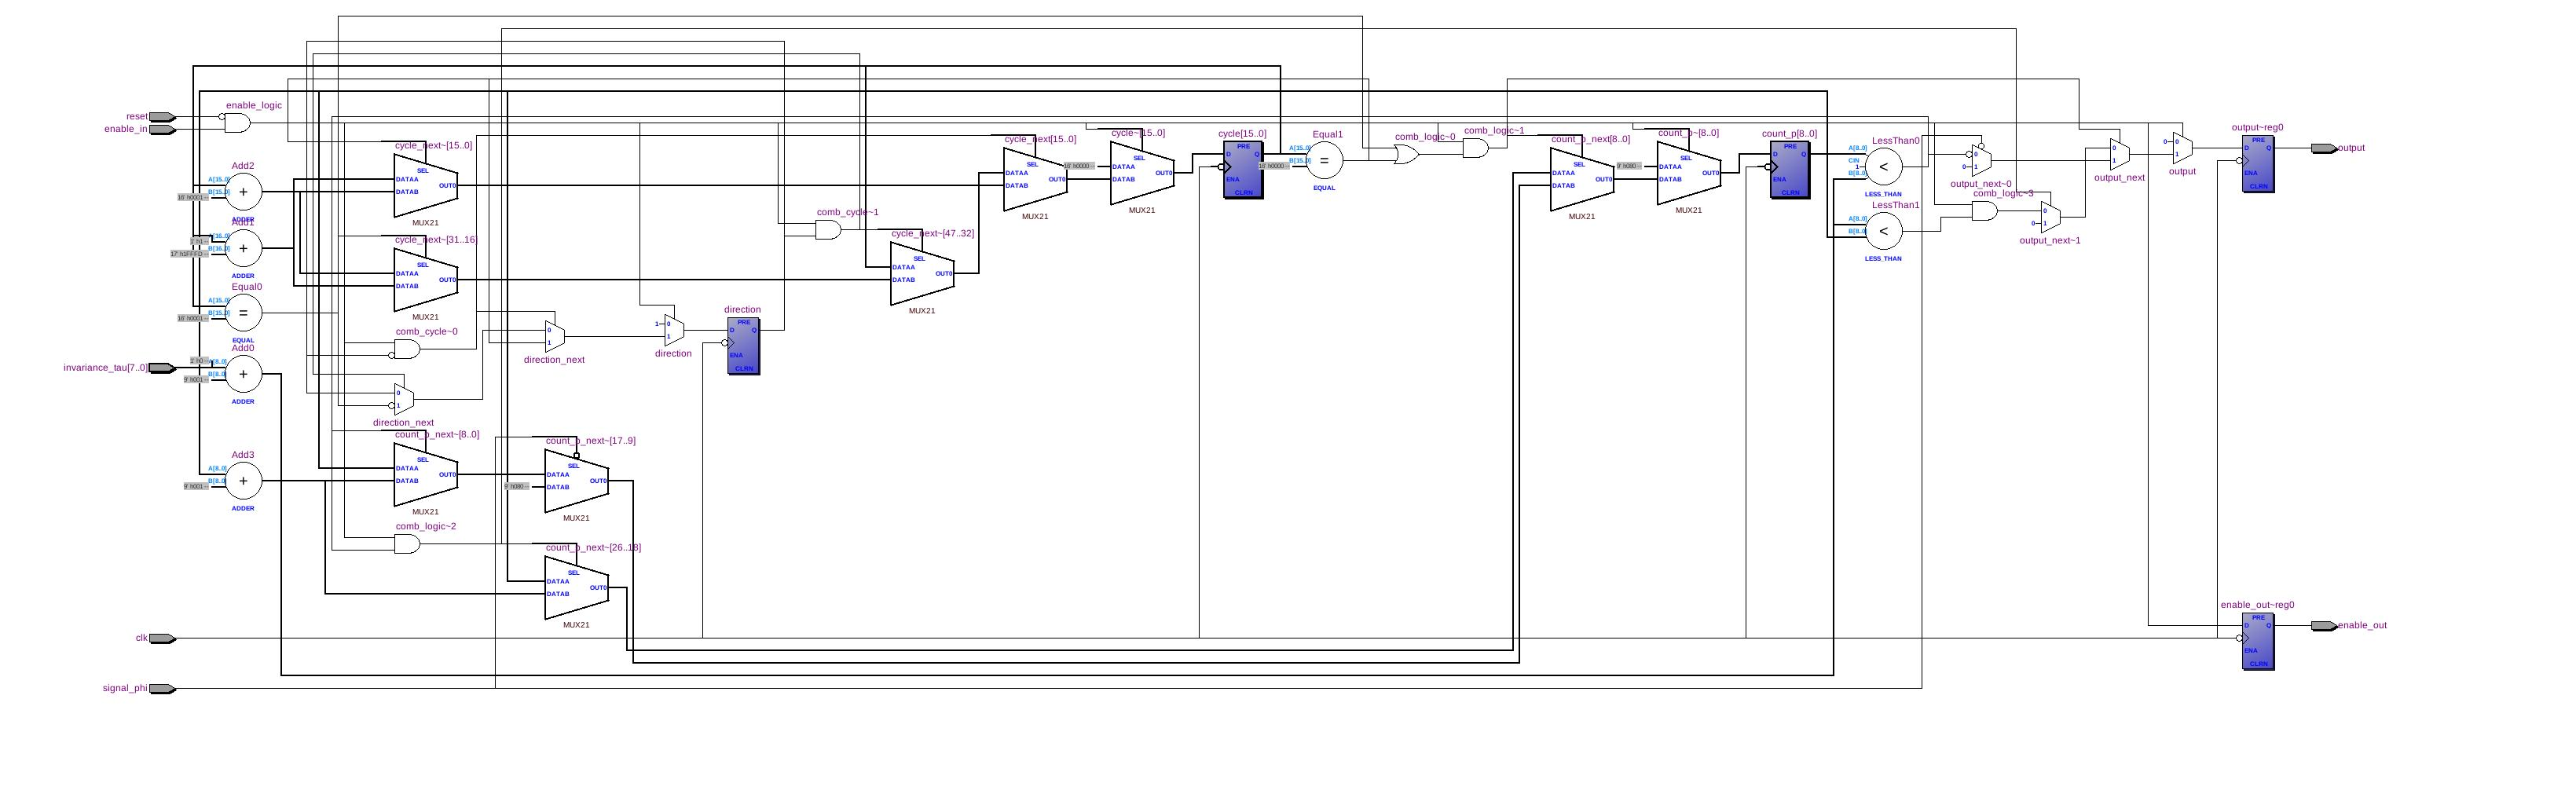
\includegraphics[width=650px,height=300px,angle=-90]{../../pictures/22.02.2014/onlyObserver/OBS_50M.jpg}
\caption[RTL View of Observer 0 with clock 50Mhz]{Shows a RTL View of a single observer stage with input clock of 50Mhz}
\label{fig:test:only:50:obs0}
\end{figure}

\begin{figure}[]
\centering
%\hspace{3.0cm}
%\vspace{-5cm}
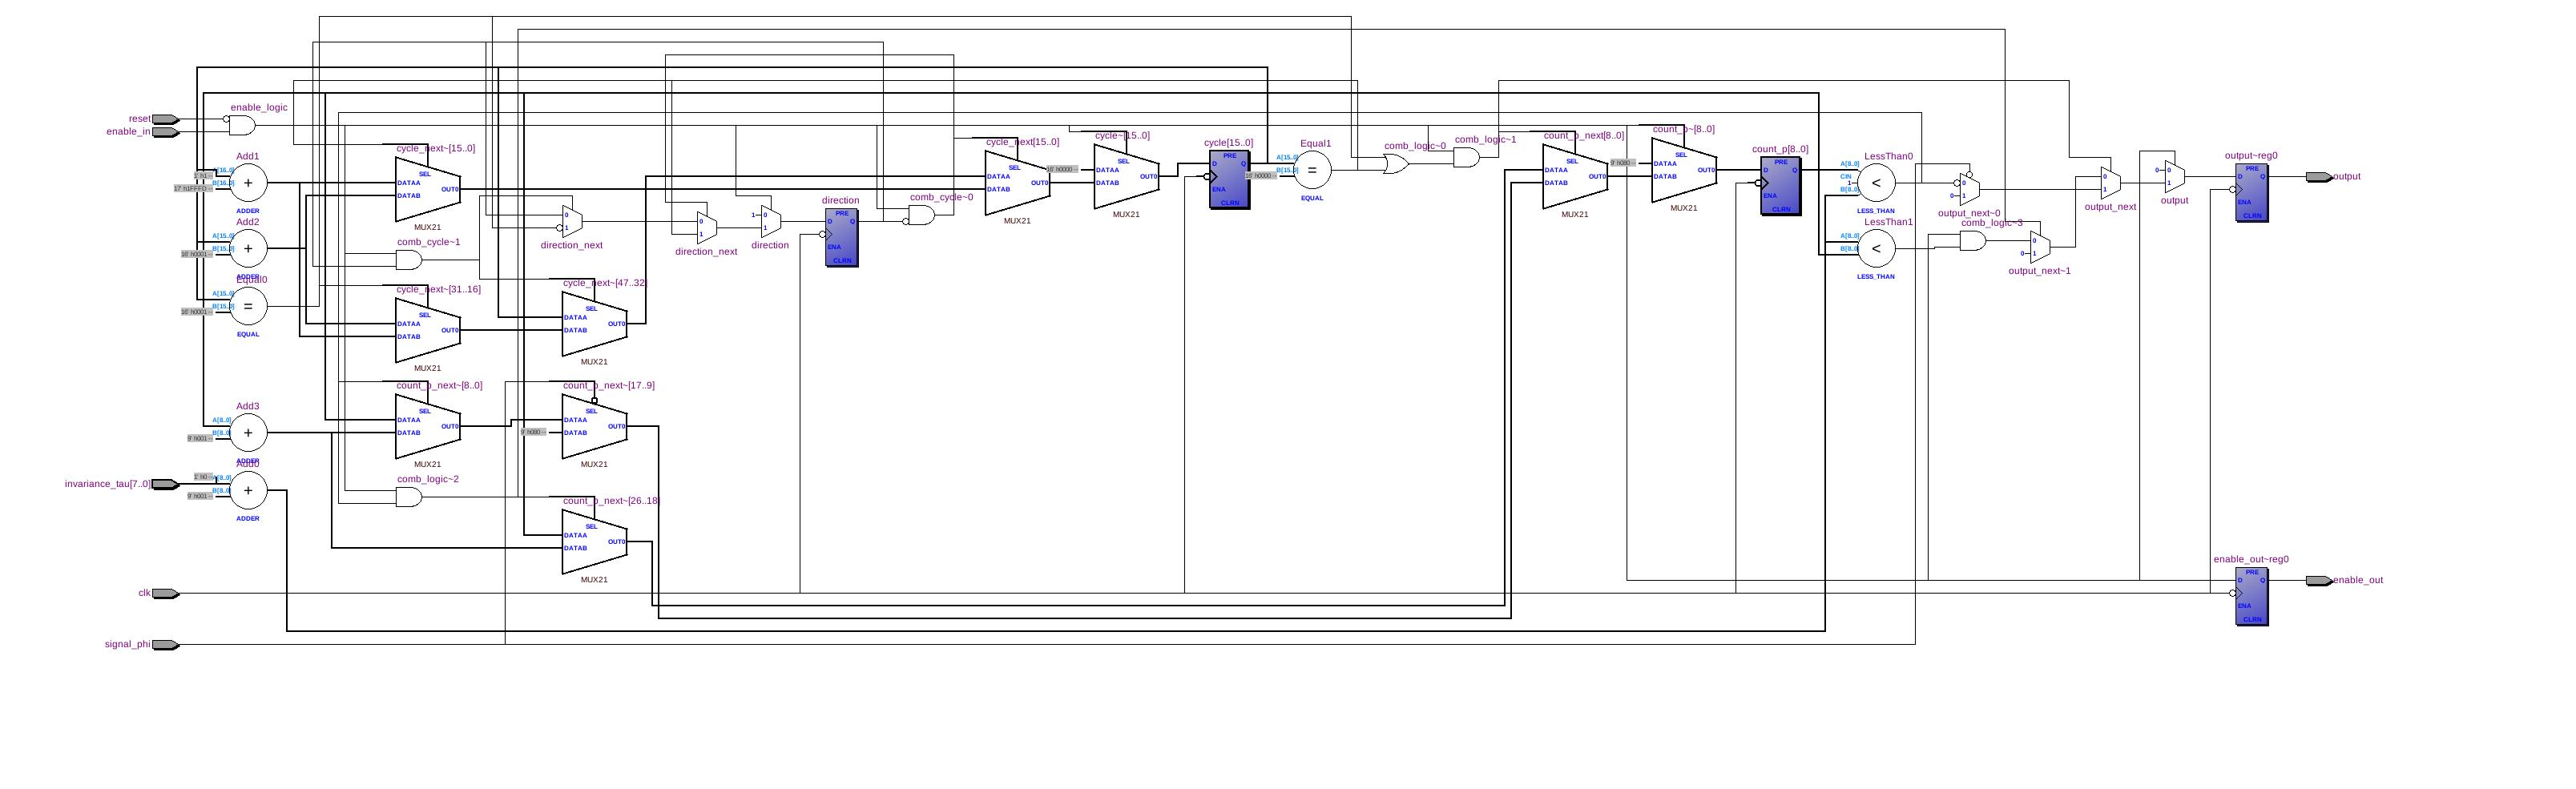
\includegraphics[width=650px,height=300px,angle=-90]{../../pictures/22.02.2014/onlyObserver/OBS_150M.jpg}
\caption[RTL View of Observer 0 with clock 150Mhz]{Shows a RTL View of a single observer stage with input clock of 150Mhz}
\label{fig:test:only:150:obs0}
\end{figure}

\newpage
\section{Design problems in the development}

This subsection is only a kind of a protocoll about problems during the development.
\begin{enumerate}
\item The starting condition of the Algorithm~\ref{alg:observerstage} was uncertain,the question was,should variable
count be initialised with 0 ot with ($\tau + 1$).If count=($\tau + 1$) then the output is immediately switched on,which
correspond to an invariance qualification.If we go back to the specification of an observer from \cite{RTFMBJ13},we know from
the proof of Theorem1(in \cite{RTFMBJ13}) that $\forall i:(i \in [max(0,n-\tau),n] \rightarrow e^i \models \phi)$ which follows 
that at the beginning of an execution if $ni-\tau$ exceeds th bottom border,but the signal $\phi$ is true,the invariance qualification
is fulfilled by that specification. 
This condition only holds if signal $\phi$ is knows at that time,in our case the status of signal $\phi$ is always(if $m \ge 1$) taken from the past.
So it is not known which status signal $\phi$ has before execution time $e^0$.Hence,we initialised the Algorithm~\ref{alg:observerstage} in a kind of,so that
no decisions about invariance qualification can made.
\item I tested the Invariance Observer with a  self-made signalgenerator which imitates input $\phi$.As a result,I created two clock domains,although the clock signals
came from the same PLL(Phase Locked Loop).If one clock is an "even" multiple of the other clock frequency,there was no problem,but if the clock frequencies are choosed in a different way,then
it comes to clock drifts.
\item The file (*.sdc file)for timings must always be adjusted,if there are changes in one of the clock domains.The PLL output Timings have to be analyzed separately by the
TimeQuest Timing Analyzer.If this does not happen,you get false estimations for "Slow 1200mv 85°C model" maximum frequencies and worst case paths.
\item The first download of the compliated design to the FPGA was no succesfull,because the Quartus Tool was not correctly adjusted to that plattfom.
Following points have to be changed:
\begin{itemize}
\item The correct architecture must be set
\item the voltage must be set for all inputs and outputs
\end{itemize}
\item Always consider what is the active state of an input component or output component,for example
input KEY is low active and was used for reseting the board. 
\end{enumerate}
